% !TEX TS-program = pdflatex
% !TEX encoding = UTF-8 Unicode

% This is a simple template for a LaTeX document using the "article" class.
% See "book", "report", "letter" for other types of document.

% Rantanen: Might prefer 'report' document type. Mainly for the use of Chapters.

\documentclass[11pt]{article} % use larger type; default would be 10pt

\usepackage[utf8]{inputenc} % set input encoding (not needed with XeLaTeX)

%%% Examples of Article customizations
% These packages are optional, depending whether you want the features they provide.
% See the LaTeX Companion or other references for full information.

%%% PAGE DIMENSIONS
\usepackage{geometry} % to change the page dimensions
\geometry{a4paper} % or letterpaper (US) or a5paper or....
% \geometry{margins}{2cm} % for example, change the margins to 2 inches all round
% \geometry{landscape} % set up the page for landscape
%   read geometry.pdf for detailed page layout information

\usepackage{graphicx} % support the \includegraphics command and options
\usepackage{hyperref}

\usepackage[parfill]{parskip} % Activate to begin paragraphs with an empty line rather than an indent

%%% PACKAGES
\usepackage{booktabs} % for much better looking tables
\usepackage{array} % for better arrays (eg matrices) in maths
\usepackage{paralist} % very flexible & customisable lists (eg. enumerate/itemize, etc.)
\usepackage{verbatim} % adds environment for commenting out blocks of text & for better verbatim
\usepackage{subfig} % make it possible to include more than one captioned figure/table in a single float
% These packages are all incorporated in the memoir class to one degree or another...

% Colored tables
\usepackage{color}
\usepackage{colortbl}

\usepackage{mathtools}
\usepackage{amssymb}

\DeclareMathOperator{\bit}{bit}
\DeclareMathOperator{\band}{and}
\DeclareMathOperator{\lshift}{<<}
\DeclareMathOperator{\rshift}{>>}
\DeclareMathOperator{\append}{\triangleright}

% Configure fancyvrb for our listings
\usepackage{fancyvrb}
\fvset{frame=leftline, framesep=5mm, tabsize=8, numbers=left}

%%% HEADERS & FOOTERS
\usepackage{fancyhdr} % This should be set AFTER setting up the page geometry
\pagestyle{fancy} % options: empty , plain , fancy
\renewcommand{\headrulewidth}{0pt} % customise the layout...
\lhead{}\chead{}\rhead{}
\lfoot{}\cfoot{\thepage}\rfoot{}

%%% SECTION TITLE APPEARANCE
\usepackage{sectsty}
\allsectionsfont{\sffamily\mdseries\upshape} % (See the fntguide.pdf for font help)
% (This matches ConTeXt defaults)

%%% ToC (table of contents) APPEARANCE
\usepackage[nottoc,notlof,notlot]{tocbibind} % Put the bibliography in the ToC
\usepackage[titles,subfigure]{tocloft} % Alter the style of the Table of Contents
\renewcommand{\cftsecfont}{\rmfamily\mdseries\upshape}
\renewcommand{\cftsecpagefont}{\rmfamily\mdseries\upshape} % No bold!

%%% END Article customizations

%%% The "real" document content comes below...

\title{Mumble protocol 1.2.X reference (WIP)}
\author{Stefan Hacker, Mikko Rantanen}
%\date{} % Activate to display a given date or no date (if empty),
         % otherwise the current date is printed 

\newenvironment{mumbleMessage}[1]
{%
\begin{center}
	\begin{tabular}{|p{0.2\textwidth}|p{0.2\textwidth}|}
	%\begin{tabular}{|l|l|}
	\hline
	\multicolumn{2}{|>{\columncolor[rgb]{0.5,0.75,1}}l|}{\textbf{#1}} \\
	\hline
}
{%
	\\ \hline
	\end{tabular}
\end{center}
}

\newenvironment{mumbleMessageEx}
{%
	\small
	\renewcommand\arraystretch{1.5}
	\begin{tabular}{p{0.25\linewidth}p{0.13\linewidth}p{0.05\linewidth}p{0.45\linewidth}}
	Field & Type & Rule & Description \\
	\hline
}
{%
	\end{tabular}
	\renewcommand\arraystretch{1.0}
}

\newcommand{\mumbleMessageExItem}[4]{ \texttt{#1} & \texttt{#2} & #3 & #4 \\ }

\newenvironment{mumbleEnum}
{%
	\small
	\renewcommand\arraystretch{1.5}
	\begin{tabular}{p{0.25\linewidth}p{0.13\linewidth}p{0.4\linewidth}}
	Name & Value & Description \\
	\hline
}
{%
	\end{tabular}
	\renewcommand\arraystretch{1.0}
}

\newcommand{\mumbleEnumItem}[3]{ \texttt{#1} & \texttt{#2} & #3 \\ }


\begin{document}
\maketitle

\newpage
\section*{DISCLAIMER}

THIS DOCUMENTATION IS PROVIDED BY THE MUMBLE PROJECT "AS IS" AND ANY EXPRESS OR IMPLIED WARRANTIES, INCLUDING, BUT NOT LIMITED TO, THE IMPLIED WARRANTIES OF MERCHANTABILITY AND FITNESS FOR A PARTICULAR PURPOSE ARE DISCLAIMED. IN NO EVENT SHALL THE MUMBLE PROJECT BE LIABLE FOR ANY DIRECT, INDIRECT, INCIDENTAL, SPECIAL, EXEMPLARY, OR CONSEQUENTIAL DAMAGES (INCLUDING, BUT NOT LIMITED TO, PROCUREMENT OF SUBSTITUTE GOODS OR SERVICES; LOSS OF USE, DATA, OR PROFITS; OR BUSINESS INTERRUPTION) HOWEVER CAUSED AND ON ANY THEORY OF LIABILITY, WHETHER IN CONTRACT, STRICT LIABILITY, OR TORT (INCLUDING NEGLIGENCE OR OTHERWISE) ARISING IN ANY WAY OUT OF THE USE OF THIS DOCUMENTATION, EVEN IF ADVISED OF THE POSSIBILITY OF SUCH DAMAGE. 

\tableofcontents
\newpage

\section{Introduction}
This document is meant to be a reference for the Mumble VoIP 1.2.X server-client communication protocol. It reflects the state of the protocol implemented in the Mumble 1.2.2 client and might be outdated by the time you are reading this. Be sure to check for newer revisions of this document on our website \url{http://www.mumble.info} . At the moment this document is work in progress.

\section{Overview}

\begin{figure}[ht]
	\centering
	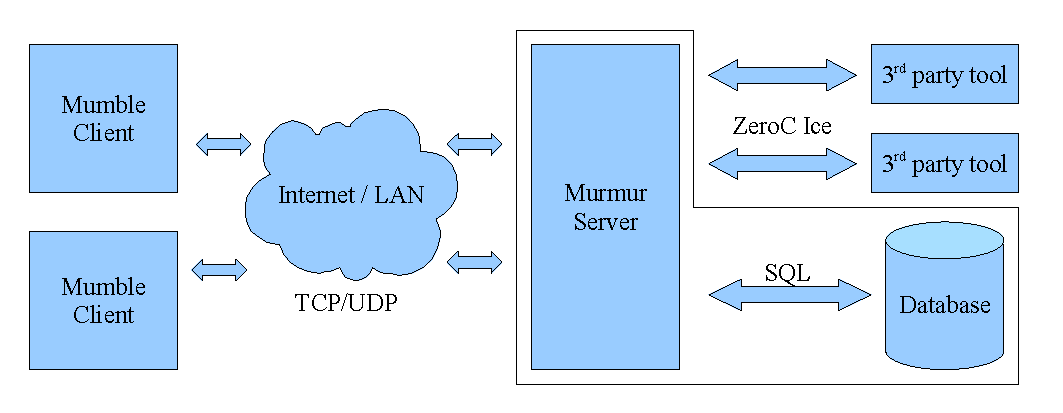
\includegraphics[width=\linewidth]{resources/mumble_system_overview}
	\caption{Mumble system overview}
	\label{fig:mumble_system_overview}
\end{figure}

Mumble is based on a standard server-client communication model. It utilizes two channels of communication, the first one is a TCP connection which is used to reliably transfer control data between the client and the server. The second one is a UDP connection which is used for unreliable, low latency transfer of voice data.

\begin{figure}[ht]
	\centering
	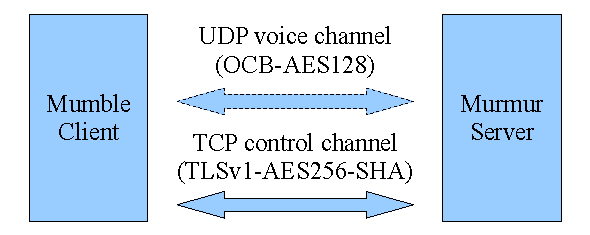
\includegraphics[width=0.5\linewidth]{resources/mumble_crypt_types}
	\caption{Mumble crypto types}
	\label{fig:mumble_crypt_types}
\end{figure}

Both are protected by strong cryptography, this encryption is mandatory and cannot be disabled. The TCP control channel uses TLSv1 AES256-SHA\footnote{\url{http://en.wikipedia.org/wiki/Transport_Layer_Security }} while the voice channel is encrypted with OCB-AES128\footnote{\url{http://www.cs.ucdavis.edu/~rogaway/ocb/ocb-back.htm}}.

While the TCP connection is mandatory the UDP connection can be compensated by tunnelling the UDP packets through the TCP connection as described in the protocol description later.

\section{Protocol stack (TCP)}

\begin{figure}[ht]
	\centering
	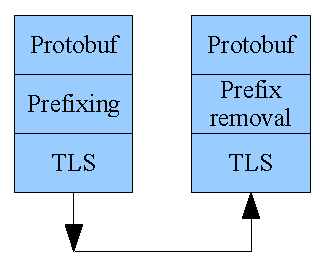
\includegraphics[width=0.3\linewidth]{resources/mumble_protocol_stack}
	\caption{Mumble protocol stack}
	\label{fig:mumble_protocol_stack}
\end{figure}

Mumble has a shallow and easy to understand stack. Basically it uses Google's Protocol Buffers\footnote{\url{http://code.google.com/p/protobuf/}} with simple prefixing to distinguish the different kinds of packets sent through an TLSv1 encrypted connection. This makes the protocol very easily expandable.

\begin{figure}[ht]
	\centering
	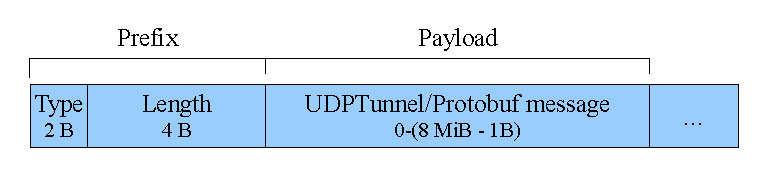
\includegraphics[width=0.8\linewidth]{resources/mumble_packet}
	\caption{Mumble packet}
	\label{fig:mumble_packet}
\end{figure}

The prefix consists out of the two bytes defining the type of the packet in the payload and 4 bytes stating the length of the payload in bytes followed by the payload itself. The following packet types are available in the current protocol and all but UDPTunnel are simple protobuf messages. If not mentioned otherwise all fields are little-endian encoded.

%FIGURE GOES HERE

For raw representation of each packet type see the attached Mumble.proto file.

\section{Establishing a connection}
This section describes the communication between the server and the client during connection establishing, note that only the TCP connection needs to be established for the client to be connected. After this the client will be visible to the other clients on the server and able to send other types of messages.

\begin{figure}[ht]
	\centering
	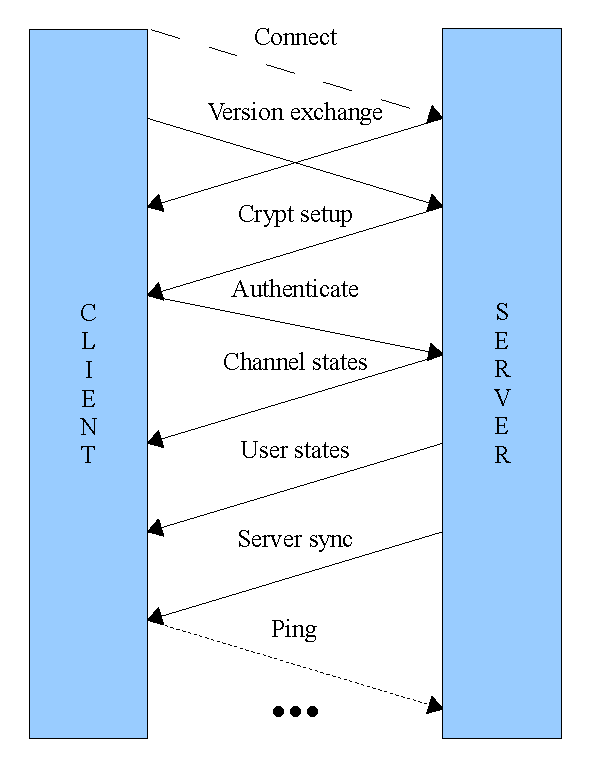
\includegraphics[width=0.7\linewidth]{resources/mumble_connection_setup}
	\caption{Mumble connection setup}
	\label{fig:mumble_connection_setup}
\end{figure}

\subsection{Connect}
As the basis for the synchronization procedure the client has to first establish the TCP connection to the server and do a common TLSv1 handshake. To be able to use the complete feature set of the Mumble protocol it is recommended that the client provides a strong certificate to the server. This however is not mandatory as you can connect to the server without providing a certificate. However the server must provide the client with its certificate and it is recommended that the client checks this.

\subsection{Version exchange}
Once the TLS handshake is completed both sides should transmit their version information using the Version message. The message structure is described below.

\begin{figure}[htp]\begin{center}

\begin{mumbleMessage}{Version}
	version		& uint32 \\
	release		& string \\
	os			& string \\
	os\_version	& string
\end{mumbleMessage}

\caption{Version message}\label{msg:conn:version}
\end{center}\end{figure}

The version field is a combination of major, minor and patch version numbers (e.g. 1.2.0) so that major number takes two bytes and minor and patch numbers take one byte each. The structure is shown in figure \ref{fig:versionEncoding}. The release, os and os\_version fields are common strings containing additional information. This information is not interpreted in any way at the moment.

\begin{figure}[htp]\begin{center}\begin{tabular}{|@{\hspace{0.5cm}}c@{\hspace{0.5cm}}|c|c|}

\hline
Major	& Minor	& Patch \\
2B		& 1B	& 1B \\
\hline

\end{tabular}

\caption{\texttt{version} field structure}\label{fig:versionEncoding}

\end{center}\end{figure}

\subsection{Authenticate}
Once the client has sent the version it should follow this with the Authenticate message. The message structure is described below in figure \ref{msg:conn:authenticate}. This message may be sent immediately after sending the version message. The client does not need to wait for the server version message.

\begin{figure}[htp]\begin{center}
\begin{mumbleMessage}{Authenticate}
	username	& string \\
	password	& string \\
	tokens		& repeated string
\end{mumbleMessage}
\caption{Authenticate message}\label{msg:conn:authenticate}
\end{center}\end{figure}

The username and password are UTF-8 encoded strings. While the client is free to accept any username from the user the server is allowed to impose further restrictions. Furthermore if the client certificate has been registered with the server the client is primarily known with the username they had when the certificate was registered. For more information see the server documentation.

The password must only be provided if the server is passworded, the client provided no certificate but wants to authenticate to an account which has a password set, or to access the SuperUser account.

The third field contains a list of zero or more token strings which act as passwords that may give the client access to certain ACL groups without actually being a registered member in them, again see the server documentation for more information.

\subsection{Crypt setup}
Once the Version packets are exchanged the server will send a CryptSetup packet to the client. It contains the necessary cryptographic information for the OCB-AES128 encryption used in the UDP Voice channel. The packet is described in figure \label{msg:conn:cryptSetup}. The encryption itself is described later in section \ref{sect:udpEncryption}.

\begin{figure}[htp]\begin{center}
\begin{mumbleMessage}{CryptSetup}
	key				& bytes \\
	client\_nonce	& bytes \\
	server\_nonce	& bytes
\end{mumbleMessage}

\caption{CryptSetup message}\label{msg:conn:cryptSetup}
\end{center}\end{figure}

\subsection{Channel states}
\label{sect:conn:channels}

After the client has successfully authenticated the server starts listing the channels by transmitting partial ChannelState message for every channel on this server. These messages lack the channel link information as the client does not yet have full picture of all the channels. Once the initial ChannelState has been transmitted for all channels the server updates the linked channels by sending new packets for these. The full structure of these ChanneLState messages is shown in \ref{msg:conn:channelState}.

\begin{figure}[htp]\begin{center}
\begin{mumbleMessage}{ChannelState}
	channel\_id	& uint32 \\
	parent		& uint32 \\
	name		& string \\
	links		& uint32, repeated \\
	description	& string \\
	links\_add	& uint32, repeated \\
	links\_remove	& uint32, repeated \\
	temporary	& bool, optional \\
	position	& int32, optional
\end{mumbleMessage}
\caption{ChannelState message}\label{msg:conn:channelState}
\end{center}\end{figure}

\emph{The server must send a ChannelState for the root channel identified with ID 0.}

\subsection{User states}
\label{sect:conn:users}

After the channels have been synchronized the server continues by listing the connected users. This is done by sending a UserState message for each user currently on the server, including the user that is currently connecting. The message structure is shown in figure \ref{msg:conn:userState}.

\begin{figure}[htp]\begin{center}
\begin{mumbleMessage}{ChannelState}
session			& uint32 \\
actor			& uint32 \\
name			& string \\
user\_id		& uint32 \\
channel\_id		& uint32 \\
mute			& bool \\
deaf			& bool \\
suppress		& bool \\
self\_mute		& bool \\
self\_deaf		& bool \\
texture			& bytes \\
plugin\_context	& bytes \\
plugin\_identity	& string \\
comment			& string \\
hash			& string \\
comment\_hash	& bytes \\
texture\_hash	& bytes \\
priority\_speaker	& bool \\
recording		& bool
\end{mumbleMessage}
\caption{UserState message}\label{msg:conn:userState}
\end{center}\end{figure}


\subsection {Server sync}
\label{sect:serverSync}

The client has now received a copy of the parts of the server state he needs to know about. To complete the synchronization the server transmits a ServerSync message containing the session id of the clients session, the maximum bandwidth allowed on this server, the servers welcome text as well as the permissions the client has in the channel he ended up.

%FIGURE GOES HERE
For more information pease refer to \nameref{appendix:mumble_proto} in the appendix.

\subsection {Ping}

If the client wishes to maintain the connection to the server it is required to ping the server. If the server does not receive a ping for 30 seconds it will disconnect the client.

\section {Voice data}

\subsection{Enabling the UDP channel}
\label{sect:udpping}

Before the UDP channel can reliably be used both sides should be certain that the connection works. Before the server may use the UDP connection to the client the client must first open a UDP socket and communicate its address to the server by sending a packet over UDP. Once the server has received an UDP transmission the server should start using the UDP channel for the voice packets. Respectively the client should not use the UDP channel for voice data until it is certain that the packets go through to the server.

In practice these requirements are filled with UDP ping. When the server receives a UDP ping packet (See figure \ref{fig:udpping}) from the client it echoes the packet back. When the client receives this packet it can ascertain that the UDP channel works for two-way communication.

\begin{figure}[htp]\begin{center}\begin{tabular}{|rcl|p{0.3\textwidth}}

\cline{1-3}
byte &:& type/flags & \texttt{0010 0000} for Ping \\
\cline{1-3}
varint &:& timestamp & Timestamp for the client. \\
\cline{1-3}

\end{tabular}
\caption{UDP Ping packet}\label{fig:udpping}
\end{center}\end{figure}

If the client stops receiving replies to the UDP packets at some point or never receives the first one it should immediately start tunneling the voice communication through TCP as described in section \ref{sect:udptunnel}. When the server receives a tunneled packet over the TCP connection it must also stop using the UDP for communication. The client may continue sending UDP ping packets over the UDP channel and the server must echo these if it receives them. If the client later receives these echoes it may switch back to the UDP channel for voice communication. When the server receives a UDP voice communication packet from the client it should stop tunneling the packets as well.

\subsection{Data}

The voice data is transmitted in variable length packets that consist of header portion, followed by repeated data segments and an optional position part. The full packet structure is shown in figure \ref{fig:udpvoice}. The decrypted data should never be longer than 1020 bytes, this allows the use of 1024 byte UDP buffer even after the 4-byte encryption header is added to the packet during the encryption. The protocol transfers 64-bit integers using variable length encoding. This encoding is specified in section \ref{sect:varint}.

\begin{figure}[htp]\begin{center}\begin{tabular}{l|rcl|p{0.5\textwidth}}

\cline{2-4}
\textbf{Header} & byte &:& type/target & Bit 1-3: Type, Bit 4-8: Target \\
				\cline{2-4}
				& varint &:& session & The session number of the source user \\
				\cline{2-4}
				& varint &:& sequence & \\
				\cline{2-4}
\multicolumn{5}{c}{} \\
				\cline{2-4}
\textbf{Audio}	& byte &:& header & Bit 1: Terminator, Bit 2-8: Data length \\
				\cline{2-4}
Repeated		& byte[] &:& data & Encoded voice frames\\
				\cline{2-4}
\multicolumn{5}{c}{} \\
				\cline{2-4}

\textbf{Position} & float &:& Pos 1 & Positional audio positions \\
				\cline{2-4}
Optional		& float &:& Pos 2 & Uses PacketDataStream encoding \\
				\cline{2-4}
				& float &:& Pos 3 & \\
				\cline{2-4}

\end{tabular}
\caption{UDP Voice packet}\label{fig:udpvoice}
\end{center}\end{figure}

The first byte of the header contains the packet type and additional target specifier. The type is stored in the first three bits and specifies the type and encoding of the packet. Current types are listed in table \ref{tbl:udptypes}. The remaining 5 bits specify additional packet-wide options. For voice packets the values specify the voice target as listed in table \ref{tbl:udptargets}.

\begin{table}[htp]\begin{center}
	\caption{UDP Types}\label{tbl:udptypes}

	\begin{tabular}{ll}
		Type & Description \\
		\hline
		0	& CELT Alpha encoded voice data \\
		1	& Ping packet (See section \ref{sect:udpping}) \\
		2	& Speex encoded voice data \\
		3	& CELT Beta encoded voice data \\
		4-7 & Unused
	\end{tabular}
\end{center}\end{table}

\begin{table}[htp]\begin{center}
	\caption{UDP targets}\label{tbl:udptargets}

	\begin{tabular}{ll}
		Target & Description \\
		\hline
		0	& Normal talking \\
		1	& Whisper to channel \\
		2-30	& Direct whisper \\
			& Always 2 for incoming whisper. \\
		31	& Server loopback
	\end{tabular}
\end{center}\end{table}

The audio frames consist of one byte long header and up to 127 bytes long data portion. The first bit in the header is the \texttt{Terminator bit} which informs the receiver whether there are more audio frames after this one. This bit is turned on (value \texttt{1}) for all but the last frame in the current UDP packet. Rest of the seven bits in the header specify the length of the data portion. The data portion is encoded using one of the supported codecs. The exact codec is specified in the type portion of the whole packet (See table \ref{tbl:udptypes}). \emph{The data in each frame is encoded separately.}

\subsubsection{Whispering}
\label{sect:whispering}

Normal talking can be heard by the users of the current channel and all linked channels as long as the speaker has Talk permission on these channels. If the speaker wishes to broadcast the voice to specific users or channels, he may use whispering. This is achieved by registering a voice target using the VoiceTarget message (See \ref{msg:voiceTarget}) and specifying the target ID as the target in the first byte of the UDP packet.

\subsection {\texttt{varint}, 64-bit integer encoding}
\label{sect:varint}

The variable length integer encoding is used to encode long, 64-bit, integers so that short values do not need the full 8 bytes to be transferred. The basic idea behind the encoding is prefixing the value with a length prefix and then removing the leading zeroes from the value. The positive numbers are always right justified. That is to say that the least significant bit in the encoded presentation matches the least significant bit in the decoded presentation. Table \ref{tbl:varint} contains the definitions of the different length prefixes. The encoded \texttt{x} bits are part of the decoded number while the \texttt{\_} signifies a unused bit. Encoding should be done by searching the first decoded description that fits the number that should be decoded, truncating it to the required bytes and combining it with the defined encoding prefix. 

\begin{table}[htp]\begin{center}
	\caption{\texttt{varint} prefixes}\label{tbl:varint}

	\begin{tabular}{ll}
		Encoded & Decoded \\
		\hline
		\texttt{0xxxxxxx} & 1 byte with $7 \cdot 8 + 1$ leading zeroes \\
		\texttt{10xxxxxx} + 1 byte & 2 bytes with $6 \cdot 8 + 2$ leading zeroes \\
		\texttt{110xxxxx} + 2 bytes & 3 bytes with $5 \cdot 8 + 3$ leading zeroes \\
		\texttt{1110xxxx} + 3 bytes & 4 bytes with $4 \cdot 8 + 4$ leading zeroes \\
		\texttt{111100\_\_} + \texttt{int} (4 bytes) & 32-bit positive number \\
		\texttt{111101\_\_} + \texttt{long} (8 bytes) & 64-bit number \\
\\
		\texttt{111110\_\_} + \texttt{varint} & Negative \texttt{varint} \\
		\texttt{111111xx} & Negative two byte number (-xx) \\
	\end{tabular}
\end{center}\end{table}

% The variable length integer encoding is used to encode long (64-bit) integers so that short values do not need the full 8 bytes to be transferred. The encoding function is given below. While it might seem complex it is worth noting that the $(a_v, a_p) \append (b_v, b_p)$ function equals appending the $a_p$ bits long value $a_v$ to a byte stream that already has the $b_p$ bits long value $b_v$.

% Encoding function
% \begin{align*}
% 	(a_v, a_p) \append (b_v, b_p) &= (2^{b_p} a_v + b_v, a_p + b_p) \\
% %
% 	e &: \mathbb{N} \rightarrow \mathbb{N}_{\geq0}^2 \\
% 	e(x) &= \begin{dcases*}
% 			e_+(x, 1)										& when $ 0 \leq x < 2^{28} $ \\
% 			\left((2^8 - 2^4) \cdot {2^8}^4 + x, 2^{40}\right)			& when $ 2^{28} \leq x < 2^{32} $ \\
% 			\left((2^8 - 2^4 + 2^2) \cdot {2^8}^8 + x, 2^{72}\right)	& when $ 2^{32} \leq x $ \\
% 			(2^8 - 2^2 - x, 8)								& when $ -4 < x < 0 $ \\
% 			(2^8 - 2^3, 8) \append e(-x)					& when $ x \leq -4 $ \\
% 		\end{dcases*} \\
% %
% 	e_+(x, b) &= \begin{dcases*}
% 			(p(b) + x, 8)												& when $ r < 2^(8-b) $ \\
% 			e_+\left(\left\lfloor \frac{x}{2^8} \right\rfloor, b + 1\right) \append (x \bmod 2^8, 8)	& when $ r \geq 2^(8-b) $
% 		\end{dcases*} \\
% %
% 	p(b) &= 2^8 - 2^{9-b}
% \end{align*}

% Decoding is performed by analyzing the first byte after which the rest of the number can be read from the byte stream.

% Decoding function
% \begin{align*}
% 	s_0(x) &= 8 - \left\lfloor log_2(2^8-1 - x) \right\rfloor \\
% %
% 	f_x &: \mathbb{N}_{\geq0} \rightarrow [0, 2^8) \\
% 	d &: f \rightarrow \mathbb{N}, f = \{ f_1, f_2, f_3, ... \} \\
% 	d(f) &= \begin{dcases*}
% 			d_+\Big(f, s_0\big(f(0)\big)\Big)													& when $f(0) \leq 2^8 - 2^4 $ \\
% 			\sum_{i=0}^4 2^{32-8i}f(i)								& when $f(0) = 2^8 - 2^4 $ \\
% 			\sum_{i=0}^8 2^{64-8i}f(i)								& when $f(0) = 2^8 - 2^4 + 2^2 $ \\
% 			-d(g : g(n) = f(n+1))									& when $f(0) = 2^8 - 2^3 $ \\
% 			(2^8 - 2^2) - f(0)										& when $f(0) \geq 2^8 - 2^2 $ \\
% 		\end{dcases*} \\
% %
% 	d_+(f, z) &= -2^{8z - 7z} + \sum_{i=1}^z 2^{8z-8i}f(i-1)
% \end{align*}

\subsection{TCP tunnel}
\label{sect:udptunnel}

When the UDP packets are tunneled through the TCP tunnel they are prefixed with the TCP protocol header that contains the packet type and length and sent through the connection. (Figure \ref{fig:udptunnel})

\begin{figure}[htp]\begin{center}\begin{tabular}{|c|@{\hspace{0.5cm}}c@{\hspace{0.5cm}}|@{\hspace{3cm}}c@{\hspace{3cm}}|}

\hline
Type	& Length	& UDP Packet \\
1B		& 3B		& 0-1020B \\
\hline

\end{tabular}
\caption{UDP Voice packet}\label{fig:udptunnel}
\end{center}\end{figure}

\subsection{Encryption}

All the voice packets are encrypted once during transfer. The actual encryption depends on the used transport layer. If the packets are tunneled through TCP they are encrypted using the TLS that encrypts the whole TCP connection and if they are sent directly using UDP they must be encrypted using the OCB-AES128 encryption. The OCB-AES128 encryption is described in section \ref{sect:cryptostate}.

\subsection{Implementation notes}

\emph{\small{When implementing the protocol it is easier to ignore the UDP transfer layer at first and just tunnel the UDP data through the TCP tunnel. The TCP layer must be implemented for authentication in any case. Making sure that the voice transmission works before implementing the UDP protocol simplifies debugging greatly. The UDP protocol is a required part of the specification though.}}

\section{Messages}

\subsection{ACL}
\label{msg:acl}

\begin{mumbleMessageEx}
\mumbleMessageExItem{channel\_id}{uint32}{Req.}{Channel ID of the channel this message affects}
\mumbleMessageExItem{inherit\_acls}{bool}{Opt.}{True if the channel inherits its parent's ACLs, \textbf{Default: true}}
\mumbleMessageExItem{groups}{ChanGroup}{Rep.}{User group specifications}
\mumbleMessageExItem{acls}{ChanACL}{Rep.}{ACL specifications}
\mumbleMessageExItem{query}{bool}{Opt.}{True if the message is a query for ACLs instead of setting them, \textbf{Default: false}}
\end{mumbleMessageEx}

\subsubsection{ACL\_ChanACL}
\label{msg:chanACL}

\begin{mumbleMessageEx}
\mumbleMessageExItem{apply\_here}{bool}{Opt.}{True if this ACL applies to the current channel, \textbf{Default: true}}
\mumbleMessageExItem{apply\_subs}{bool}{Opt.}{True if this ACL applies to the sub channels, \textbf{Default: true}}
\mumbleMessageExItem{inherited}{bool}{Opt.}{True if the ACL has been inherited from the parent, \textbf{Default: true}}
\mumbleMessageExItem{user\_id}{uint32}{Opt.}{ID of the user that is affected by this ACL}
\mumbleMessageExItem{group}{string}{Opt.}{ID of the group that is affected by this group}
\mumbleMessageExItem{grant}{uint32}{Opt.}{Bit flag field of the permissions granted by this ACL}
\mumbleMessageExItem{deny}{uint32}{Opt.}{Bit flag field of the permissions denied by this ACL}
\end{mumbleMessageEx}

\subsubsection{ACL\_ChanGroup}
\label{msg:chanGroup}

\begin{mumbleMessageEx}
\mumbleMessageExItem{name}{string}{Req.}{Name of the channel group, UTF-8 enccoded}
\mumbleMessageExItem{inherited}{bool}{Opt.}{True if the group has been inherited from the parent. \textbf{Read only, Default: true}}
\mumbleMessageExItem{inherit}{bool}{Opt.}{True if the group members are inherited, \textbf{Default: true}}
\mumbleMessageExItem{inheritable}{bool}{Opt.}{True if the group can be inherited by sub channels, \textbf{Default: true}}
\mumbleMessageExItem{add}{uint32}{Rep.}{Users explicitly included in this group, identified by \texttt{user\_id}}
\mumbleMessageExItem{remove}{uint32}{Rep.}{Users explicitly removed from this group in this channel if the group has been inherited, identified by \texttt{user\_id}}
\mumbleMessageExItem{inherited\_members}{uint32}{Rep.}{Users inherited, identified by \texttt{user\_id}}
\end{mumbleMessageEx}


\subsection{Authenticate}
\label{msg:authenticate}

Used by the client to send the authentication credentials to the server.

\begin{mumbleMessageEx}
\mumbleMessageExItem{username}{string}{Opt.}{UTF-8 encoded username}
\mumbleMessageExItem{password}{string}{Opt.}{Server or user password}
\mumbleMessageExItem{tokens}{string}{Rep.}{Additional access tokens for server ACL groups}
\mumbleMessageExItem{celt\_versions}{int32}{Rep.}{A list of CELT bitstream version constants supported by the client.}
\end{mumbleMessageEx}

\subsection{BanList} 
\label{msg:banList}

Relays information on the bans. The client may send the BanList message to either modify the list of bans or query them from the server. The server sends this list only after a client queries for it.

\begin{mumbleMessageEx}
\mumbleMessageExItem{bans}{BanEntry}{Rep.}{List of ban entries currently in place}
\mumbleMessageExItem{query}{bool}{Opt.}{True if the server should return the list, False if it should replace old ban list with this one, \textbf{Default: false}}
\end{mumbleMessageEx}

\subsubsection{BanList\_BanEntry}
\label{msg:banEntry}

\begin{mumbleMessageEx}
\mumbleMessageExItem{address}{bytes}{Req.}{Banned IP address}
\mumbleMessageExItem{mask}{uint32}{Req.}{The length of the subnet mask for the ban}
\mumbleMessageExItem{name}{string}{Opt.}{User name for identification purposes, does not affect the ban}
\mumbleMessageExItem{hash}{string}{Opt.}{TODO ??}
\mumbleMessageExItem{reason}{string}{Opt.}{Reason for the ban, does not affect the ban}
\mumbleMessageExItem{start}{string}{Opt.}{Ban start time}
\mumbleMessageExItem{duration}{uint32}{Opt.}{Ban duration in seconds}
\end{mumbleMessageEx}

\subsection{ChannelRemove}
\label{msg:channelRemove}

Sent by the client when it wants a channel removed. Sent by the server when a channel has been removed and clients should be notified.

\begin{mumbleMessageEx}
\mumbleMessageExItem{channel\_id}{uint32}{Req.}{The \texttt{channel\_id} of the channel to be removed}
\end{mumbleMessageEx}

\subsection{ChannelState}
\label{msg:channelState}

Used to communicate channel properties between the client and the server. Sent by the server during the login process (See \ref{sect:conn:channels}) or when channel properties are updated. Client may use this message to update said channel properties.

\begin{mumbleMessageEx}
\mumbleMessageExItem{channel\_id}{uint32}{Opt.}{Unique ID for the channel within the server.}
\mumbleMessageExItem{parent}{uint32}{Opt.}{\texttt{channel\_id} of the parent channel.}
\mumbleMessageExItem{name}{string}{Opt.}{Channel name, UTF-8 encoded.}
\mumbleMessageExItem{links}{uint32}{Rep.}{A collection of \texttt{channel\_id} values of the linked channels. Absent during the first channel listing (See \ref{sect:conn:channels}).}
\mumbleMessageExItem{description}{string}{Opt.}{Channel description, UTF-8 encoded. Only if the description is less than 128 bytes}
\mumbleMessageExItem{links\_add}{uint32}{Rep.}{A collection of \texttt{channel\_id} values that should be added to \texttt{links}.}
\mumbleMessageExItem{links\_remove}{uint32}{Rep.}{A collection of \texttt{channel\_id} values that should be removed from \texttt{links}.}
\mumbleMessageExItem{temporary}{bool}{Opt.}{True if the channel is temporary. \textbf{Default: false}}
\mumbleMessageExItem{position}{uint32}{Opt.}{Position weight to tweak the channel position in the channel list. \textbf{Default: 0}}
\mumbleMessageExItem{description\_hash}{bytes}{Opt.}{SHA1 hash of the description if the description is 128 bytes or more. See \ref{msg:requestBlob}}
\end{mumbleMessageEx}

\subsection{CodecVersion}
\label{msg:codecVersion}

Sent by the server to notify the users of the version of the CELT codec they should use. This may change during the connection when new users join.

\begin{mumbleMessageEx}
\mumbleMessageExItem{alpha}{int32}{Req.}{The version of the CELT Alpha codec}
\mumbleMessageExItem{beta}{int32}{Req.}{The version of the CELT Beta codec}
\mumbleMessageExItem{prefer\_alpha}{bool}{Req.}{True if the user should prefer Alpha over Beta, \textbf{Default: true}}
\end{mumbleMessageEx}

\subsection{ContextAction}
\label{msg:contextAction}

Sent by the client when it wants to initiate a Context action. Refer to Mumble documentation (TODO Context action source) for more information.

\begin{mumbleMessageEx}
\mumbleMessageExItem{session}{uint32}{Opt.}{The target User for the action, identified by \texttt{session}}
\mumbleMessageExItem{channel\_id}{uint32}{Opt.}{The target Channel for the action, identified by \texttt{channel\_id}}
\mumbleMessageExItem{action}{string}{Req.}{The action that should be executed}
\end{mumbleMessageEx}

\subsection{ContextActionAdd}
\label{msg:contextActionAdd}

Sent by the server to inform the client of available context actions.

\begin{mumbleMessageEx}
\mumbleMessageExItem{action}{string}{Req.}{The action name}
\mumbleMessageExItem{text}{string}{Req.}{The display name of the action}
\mumbleMessageExItem{context}{uint32}{Opt.}{Context bit flags defining where the action should be displayed, see \ref{msg:contextActionAdd:context}}
\end{mumbleMessageEx}

\subsubsection{Enumeration: ContextActionAdd\_Context}
\label{msg:contextActionAdd:context}

\begin{mumbleEnum}
\mumbleEnumItem{Server}{0x01}{Action is applicable to the server}
\mumbleEnumItem{Channel}{0x02}{Action can target a Channel}
\mumbleEnumItem{User}{0x04}{Action can target a User}
\end{mumbleEnum}

\subsection{CryptSetup}
\label{msg:cryptSetup}

Used to initialize and resync the UDP encryption. See section \ref{sect:encryption} for more information. Either side may request a resync by sending the message without any values filled. The resync is performed by sending the message with only the client or server nonce filled.

\begin{mumbleMessageEx}
\mumbleMessageExItem{key}{bytes}{Opt.}{Encryption key}
\mumbleMessageExItem{client\_nonce}{bytes}{Opt.}{Client nonce}
\mumbleMessageExItem{server\_nonce}{bytes}{Opt.}{Server nonce}
\end{mumbleMessageEx}

\subsection{PermissionDenied}
\label{msg:permissionDenied}

\begin{mumbleMessageEx}
\mumbleMessageExItem{permission}{uint32}{Opt.}{The denied permission when type is \texttt{Permission}}
\mumbleMessageExItem{channel\_id}{uint32}{Opt.}{\texttt{channel\_id} for the channel where the permission was denied when type is \texttt{Permission}}
\mumbleMessageExItem{session}{uint32}{Opt.}{The user who was denied permissions, identified by \texttt{session}}
\mumbleMessageExItem{reason}{string}{Opt.}{Textual reason for the denial}
\mumbleMessageExItem{type}{DenyType}{Opt.}{Type of the denial}
\mumbleMessageExItem{name}{string}{Opt.}{The name that is invalid when type is \texttt{UserName}}
\end{mumbleMessageEx}

\subsubsection{Enumeration: PermissionDenied\_DenyType}
\label{msg:permissionDenied:denyType}

\begin{mumbleEnum}
\mumbleEnumItem{Text}{0}{Operation denied for other reason, see reason field}
\mumbleEnumItem{Permission}{1}{Permissions were denied}
\mumbleEnumItem{SuperUser}{2}{Cannot modify SuperUser}
\mumbleEnumItem{ChannelName}{3}{Invalid channel name}
\mumbleEnumItem{TextTooLong}{4}{Text message too long}
\mumbleEnumItem{H9K}{5}{The flux capacitor was spelled wrong.}
\mumbleEnumItem{TemporaryChannel}{6}{Operation not permitted in temporary channel}
\mumbleEnumItem{MissingCertificate}{7}{Operation requires certificate}
\mumbleEnumItem{UserName}{8}{Invalid username}
\mumbleEnumItem{ChannelFull}{9}{Channel is full}
\end{mumbleEnum}

\subsection{PermissionQuery}
\label{msg:permissionQuery}

Sent by the client when it wants permissions for a certain channel. Sent by the server when it replies to the query or wants the user to resync all channel permissions.

\begin{mumbleMessageEx}
\mumbleMessageExItem{channel\_id}{uint32}{Opt.}{\texttt{channel\_id} of the channel for which the permissions are queried}
\mumbleMessageExItem{permissions}{uint32}{Opt.}{Channel permissions. TODO: Encoded how?}
\mumbleMessageExItem{flush}{bool}{Opt.}{True if the client should drop its current permission information for \textbf{all} channels, \textbf{Default: false}}
\end{mumbleMessageEx}

\subsection{Ping}
\label{msg:ping}

Sent by the client to notify the server that the client is still alive. Server must reply to the packet with the same timestamp and its own good/late/lost/resync numbers. None of the fields is strictly required.

\begin{mumbleMessageEx}
\mumbleMessageExItem{timestamp}{uint64}{Opt.}{Client timestamp. Server should not attempt to decode.}
\mumbleMessageExItem{good}{uint32}{Opt.}{The amount of good packets received}
\mumbleMessageExItem{late}{uint32}{Opt.}{The amount of late packets received}
\mumbleMessageExItem{lost}{uint32}{Opt.}{The amount of packets never received}
\mumbleMessageExItem{resync}{uint32}{Opt.}{The amount of nonce resyncs}
\mumbleMessageExItem{udp\_packets}{uint32}{Opt.}{The total amount of UDP packets received}
\mumbleMessageExItem{tcp\_packets}{uint32}{Opt.}{The total amount of TCP packets received}
\mumbleMessageExItem{udp\_ping\_avg}{float}{Opt.}{UDP ping average}
\mumbleMessageExItem{udp\_ping\_var}{float}{Opt.}{UDP ping variance}
\mumbleMessageExItem{tcp\_ping\_avg}{float}{Opt.}{TCP ping average}
\mumbleMessageExItem{tcp\_ping\_var}{float}{Opt.}{TCP ping variance}
\end{mumbleMessageEx}

\subsection{QueryUsers}
\label{msg:queryUsers}

Client may use this message to refresh its registered user information. The client should fill the IDs or Names of the users it wants to refresh. The server fills the missing parts and sends the message back.

\begin{mumbleMessageEx}
\mumbleMessageExItem{ids}{uint32}{Rep.}{User IDs}
\mumbleMessageExItem{names}{string}{Rep.}{User names in the same order as \texttt{ids}}
\end{mumbleMessageEx}

\subsection{Reject}
\label{msg:reject}

Sent by the server when it rejects the user connection.

\begin{mumbleMessageEx}
\mumbleMessageExItem{type}{RejectType}{Opt.}{Rejection type}
\mumbleMessageExItem{reason}{string}{Opt.}{Human readable rejection reason}
\end{mumbleMessageEx}

\subsubsection{Enumeration: Reject\_RejectType}
\label{msg:reject:rejectType}

\begin{mumbleEnum}
\mumbleEnumItem{None}{0}{TODO ??}
\mumbleEnumItem{WrongVersion}{1}{The client attempted to connect with an incompatible version}
\mumbleEnumItem{InvalidUsername}{2}{The user name supplied by the client was invalid}
\mumbleEnumItem{WrongUserPW}{3}{The client attempted to authenticate as a user with a password but it was wrong}
\mumbleEnumItem{WrongServerPW}{4}{The client attempted to connect to a passworded server but the password was wrong}
\mumbleEnumItem{UsernameInUse}{5}{Supplied username is already in use}
\mumbleEnumItem{ServerFull}{6}{Server is currently full and cannot accept more users}
\mumbleEnumItem{NoCertificate}{7}{The user did not provide a certificate but one is required}
\end{mumbleEnum}

\subsection{RequestBlob}
\label{msg:requestBlob}

Used by the client to request binary data from the server. By default large comments or textures are not sent within standard messages but instead the hash is. If the client does not recognize the hash it may request the resource when it needs it. The client does so by sending a RequestBlob message with the correct fields filled with the hashes it wants to receive. The server replies to this by sending a new UserState/ChannelState message with the resources filled even if they would normally be transmitted as hashes.

\begin{mumbleMessageEx}
\mumbleMessageExItem{session\_texture}{uint32}{Rep.}{Hashes of the requested UserState textures}
\mumbleMessageExItem{session\_comment}{uint32}{Rep.}{Hashes of the requested UserState comments}
\mumbleMessageExItem{channel\_description}{uint32}{Rep.}{Hashes of the requested ChannelState descriptions}
\end{mumbleMessageEx}

\subsection{ServerConfig}
\label{msg:serverConfig}

Sent by the server when it informs the clients on server configuration details.

\begin{mumbleMessageEx}
\mumbleMessageExItem{max\_bandwidth}{uint32}{Opt.}{The maximum bandwith the clients should use}
\mumbleMessageExItem{welcome\_text}{string}{Opt.}{Server welcome text}
\mumbleMessageExItem{allow\_html}{bool}{Opt.}{True if the server allows HTML}
\mumbleMessageExItem{message\_length}{uint32}{Opt.}{Maximum text message length}
\mumbleMessageExItem{image\_message\_length}{uint32}{Opt.}{Maximum image message length}
\end{mumbleMessageEx}

\subsection{ServerSync}
\label{msg:serverSync}

ServerSync message is sent by the server when it has authenticated the user and finished synchronizing the server state. See section \ref{sect:serverSync} for more information on the initial connection exchange.

\begin{mumbleMessageEx}
\mumbleMessageExItem{session}{uint32}{Opt.}{The \texttt{session} of the current user}
\mumbleMessageExItem{max\_bandwidth}{uint32}{Opt.}{Maximum bandwith that the user should use}
\mumbleMessageExItem{welcome\_text}{string}{Opt.}{Server welcome text}
\mumbleMessageExItem{permissions}{uint64}{Opt.}{Current user permissions TODO: Confirm??}
\end{mumbleMessageEx}

\subsection{TextMessage}
\label{msg:textMessage}

Used to send and broadcast text messages.

\begin{mumbleMessageEx}
\mumbleMessageExItem{actor}{uint32}{Opt.}{The message sender, identified by its \texttt{session}}
\mumbleMessageExItem{session}{uint32}{Rep.}{Target users for the message, identified by their \texttt{session}}
\mumbleMessageExItem{channel\_id}{uint32}{Rep.}{The channels to which the message is sent, identified by their \texttt{channel\_id}s}
\mumbleMessageExItem{tree\_id}{uint32}{Rep.}{The root channels when sending message recursively to several channels, identified by their \texttt{channel\_id}s}
\mumbleMessageExItem{message}{string}{Req.}{The UTF-8 encoded message. May be HTML if the server allows.}
\end{mumbleMessageEx}

\subsection{UDPTunnel}
\label{msg:udpTunnel}

Used to tunnel the UDP packets through the TCP channel. See section \ref{sect:udptunnel} for more information.

\begin{mumbleMessageEx}
\mumbleMessageExItem{packet}{bytes}{Req.}{The data from the UDP packet}
\end{mumbleMessageEx}

\subsection{UserList}
\label{msg:userList}

Lists the registered users

\begin{mumbleMessageEx}
\mumbleMessageExItem{users}{User}{Rep.}{A list of registered users}
\end{mumbleMessageEx}

\subsubsection{UserList\_User}
\label{msg:userList:user}

\begin{mumbleMessageEx}
\mumbleMessageExItem{user\_id}{uint32}{Req.}{Registered user ID}
\mumbleMessageExItem{name}{string}{Opt.}{Registered user name}
\end{mumbleMessageEx}

\subsection{UserRemove}
\label{msg:userRemove}

Used to communicate user leaving or being kicked. May be sent by the client when it attempts to kick a user. Sent by the server when it informs the clients that a user is not present anymore.

\begin{mumbleMessageEx}
\mumbleMessageExItem{session}{uint32}{Req.}{The user who is being kicked, identified by their \texttt{session}, not present when no one is being kicked}
\mumbleMessageExItem{actor}{uint32}{Opt.}{The user who initiated the removal. Either the user who performs the kick or the user who is currently leaving}
\mumbleMessageExItem{reason}{string}{Opt.}{Reason for the kick, stored as the ban reason if the user is banned}
\mumbleMessageExItem{ban}{bool}{Opt.}{True if the kick should result in a ban}
\end{mumbleMessageEx}

\subsection{UserState}
\label{msg:userState}

Sent by the server when it communicates new and changed users to client. First seen during login procedure (See \ref{sect:conn:users}). May be sent by the client when it wishes to alter its state.

\begin{mumbleMessageEx}
\mumbleMessageExItem{session}{uint32}{Opt.}{Unique user session ID of the user whose state this is, may change on reconnect}
\mumbleMessageExItem{actor}{uint32}{Opt.}{The \texttt{session} of the user who is updating this user}
\mumbleMessageExItem{name}{string}{Opt.}{User name, UTF-8 encoded}
\mumbleMessageExItem{user\_id}{uint32}{Opt.}{Registered user ID if the user is registered}
\mumbleMessageExItem{channel\_id}{uint32}{Opt.}{Channel on which the user is}
\mumbleMessageExItem{mute}{bool}{Opt.}{True if the user is muted by admin}
\mumbleMessageExItem{deaf}{bool}{Opt.}{True if the user is deafened by admin}
\mumbleMessageExItem{suppress}{bool}{Opt.}{True if the user has been suppressed from talking by a reason other than being muted}
\mumbleMessageExItem{self\_mute}{bool}{Opt.}{True if the user has muted self}
\mumbleMessageExItem{self\_deaf}{bool}{Opt.}{True if the user has deafened self}
\mumbleMessageExItem{texture}{bytes}{Opt.}{User image if it is less than 128 bytes}
\mumbleMessageExItem{plugin\_context}{bytes}{Opt.}{TODO ??}
\mumbleMessageExItem{plugin\_identity}{string}{Opt.}{TODO ??}
\mumbleMessageExItem{comment}{string}{Opt.}{User comment if it is less than 128 bytes}
\mumbleMessageExItem{hash}{string}{Opt.}{The hash of the user certificate}
\mumbleMessageExItem{comment\_hash}{bytes}{Opt.}{SHA1 hash of the user comment if it 128 bytes or more. See \ref{msg:requestBlob}}
\mumbleMessageExItem{texture\_hash}{bytes}{Opt.}{SHA1 hash of the user picture if it 128 bytes or more. See \ref{msg:requestBlob}}
\mumbleMessageExItem{priority\_speaker}{bool}{Opt.}{True if the user is a priority speaker}
\mumbleMessageExItem{recording}{bool}{Opt.}{True if the user is currently recording}
\end{mumbleMessageEx}

\subsection{UserStats}
\label{msg:userStats}

Used to communicate user stats between the server and clients.

\begin{mumbleMessageEx}
\mumbleMessageExItem{session}{uint32}{Opt.}{User whose stats these are}
\mumbleMessageExItem{stats\_only}{bool}{Opt.}{True if the message contains only mutable stats (packets, ping), \textbf{Default: false}}
\mumbleMessageExItem{certificates}{bytes}{Rep.}{Full user certificate chain of the user certificate in DER format} % TODO: DER format reference
\mumbleMessageExItem{from\_client}{Stats}{Opt.}{Packet statistics for packets received from the client}
\mumbleMessageExItem{from\_server}{Stats}{Opt.}{Packet statistics for packets sent by the server}
\\
\mumbleMessageExItem{udp\_packets}{uint32}{Opt.}{Amount of UDP packets sent}
\mumbleMessageExItem{tcp\_packets}{uint32}{Opt.}{Amount of TCP packets sent}
\mumbleMessageExItem{udp\_ping\_avg}{float}{Opt.}{UDP ping average}
\mumbleMessageExItem{udp\_ping\_var}{float}{Opt.}{UDP ping variance}
\mumbleMessageExItem{tcp\_ping\_avg}{float}{Opt.}{TCP ping average}
\mumbleMessageExItem{tcp\_ping\_var}{float}{Opt.}{TCP ping variance}
\\
\mumbleMessageExItem{version}{Version}{Opt.}{Client version, see \ref{msg:version}}
\mumbleMessageExItem{celt\_versions}{int32}{Rep.}{A list of CELT bitstream version constants supported by the client of this user.}
\mumbleMessageExItem{address}{bytes}{Opt.}{Client IP address}
\mumbleMessageExItem{bandwidth}{uint32}{Opt.}{Bandwith used by this client}
\mumbleMessageExItem{onlinesecs}{uint32}{Opt.}{Connection duration}
\mumbleMessageExItem{idlesecs}{uint32}{Opt.}{Duration since last activity}
\mumbleMessageExItem{strong\_certificate}{bool}{Opt.}{True if the user has a strong certificate, \textbf{Default: false}}
\end{mumbleMessageEx}

\subsubsection{UserStats\_Stats}
\label{msg:userStats:stats}

\begin{mumbleMessageEx}
\mumbleMessageExItem{good}{uint32}{Opt.}{The amount of good packets received}
\mumbleMessageExItem{late}{uint32}{Opt.}{The amount of late packets received}
\mumbleMessageExItem{lost}{uint32}{Opt.}{The amount of packets never received}
\mumbleMessageExItem{resync}{uint32}{Opt.}{The amount of nonce resyncs}
\end{mumbleMessageEx}

\subsection{Version}
\label{msg:version}

\begin{mumbleMessageEx}
\mumbleMessageExItem{version}{uint32}{Opt.}{2-byte Major, 1-byte Minor and 1-byte Patch version number}
\mumbleMessageExItem{release}{string}{Opt.}{Client release name}
\mumbleMessageExItem{os}{string}{Opt.}{Client OS name}
\mumbleMessageExItem{os\_version}{string}{Opt.}{Client OS version}
\end{mumbleMessageEx}

\subsection{VoiceTarget}
\label{msg:voiceTarget}

Sent by the client when it wants to register or clear whisper targets. See \ref{sect:whispering} for more information. \textbf{Note: The first available target ID is 1 as 0 is reserved for normal talking. Maximum target ID is 30}

\begin{mumbleMessageEx}
\mumbleMessageExItem{id}{uint32}{Opt.}{Voice target ID}
\mumbleMessageExItem{targets}{Target}{Rep.}{The receivers that this voice target includes}
\end{mumbleMessageEx}

\subsubsection{VoiceTarget\_Target}
\label{msg:voiceTarget:target}

\begin{mumbleMessageEx}
\mumbleMessageExItem{session}{uint32}{Rep.}{Users that are included as targets}
\mumbleMessageExItem{channel\_id}{uint32}{Opt.}{Channels that are included as targets}
\mumbleMessageExItem{group}{string}{Opt.}{TODO ??}
\mumbleMessageExItem{links}{bool}{Opt.}{True if the voice should follow links from the specified channel, \textbf{Default: false}}
\mumbleMessageExItem{children}{bool}{Opt.}{True if the voice should also be sent to children of the specifiec channel, \textbf{Default: false}}
\end{mumbleMessageEx}


% Right place?


\section {This document is WIP}
SORRY BUT THIS DOCUMENT IS WORK IN PROGRESS. AT THE MOMENT IT LACKS A LOT OF IMPORTANT INFORMATION BUT WE HOPE TO BE ABLE TO FINISH THIS DOCUMENT SOMEDAY :-)

\appendix
\section{Appendix}
\subsection{Mumble.proto}
\label{appendix:mumble_proto}
\VerbatimInput{../src/Mumble.proto}

\end{document}

% vim: ts=4 sw=4 noexpandtab
